% !TEX root = SystemTemplate.tex

\chapter{Design  and Implementation}
The software is designed and implemented in term of different components, and it can be splitted into GUI and database. \\


This chart is generated by power-designer and we basically built database based on this schema. There are several tables stores different information. There are Student, teacher, admins and class tables and each are connected by different relationship in order to perform certain functionalities we want. It consists many-to-many relationship has intermediate table and many-to-one relationship. We also have account table for user authentication and it has permission level included in order to distinguish different user groups for example admin and teacher have different permission levels. By the way, we are going to add new table for billing and payroll in later spring as well.\\
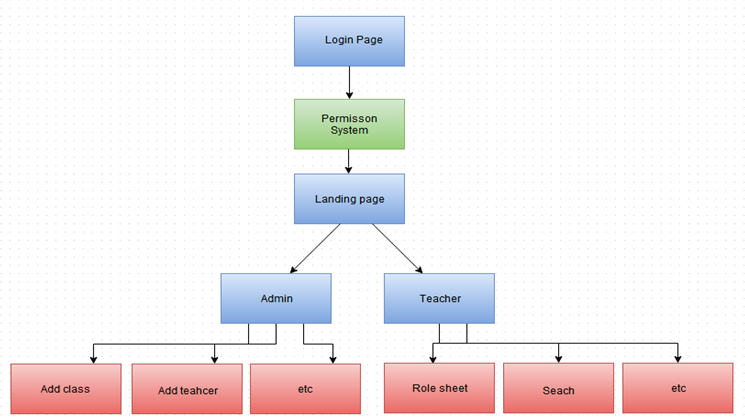
\includegraphics[scale=0.5]{pics/gui.png}\\
For the GUI part, you can see here this flow chart is our data flow for gui. Users can log into system through the login page and if username and password are correct it leads user to permission system otherwise users get rejected from system. From permission system, user either can be leaded to admin or teachers landing pages. Then if users are admins they can search employees’ information, add class, add teacher, assign teacher to class, sets clothing requirement for specific class. If users are teachers, they can search students’ information, assign students to class, print the role sheet of the class she is teaching.
In spring 3.5, we also going to add a student web interface and they can use that to register classes and check class schedule. 
\\


\section{Database}

\subsection{Technologies  Used}
We use Power Designer to generate our initial database schema and SQL scripts. Then, we put the SQL scripts MySQL workbench to generate database tables.

\subsection{Component  Overview}
There are several tables in database stores different information and interact with each other.\\
Account\\
Address\\
Admin\\
Class\\
Guardian\\
Student\\
Student\_Class\\
Teacher\\
Teacher\_Class\\

\subsection{Phase Overview}
This is an extension of the Phase Overview above, but specific to this component. 
 It is meant to be basically a brief list with space for marking the phase status. 

\subsection{ Architecture  Diagram}
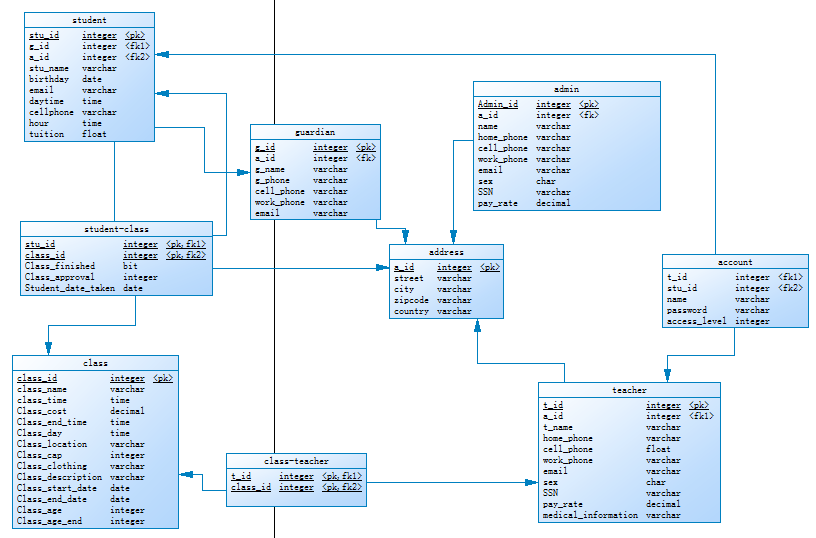
\includegraphics[scale=0.8]{pics/database.png}\\


\subsection{Data Flow Diagram}
It is important to build and maintain a data flow diagram.  However, it may be 
that a component is best described visually with an architecture diagram. 


\subsection{Design Details}
This is where the details are presented and may contain subsections.   Here is an example code listing:
\begin{lstlisting}
#include <stdio.h>
#define N 10
/* Block
 * comment */
 
int main()
{
    int i;
 
    // Line comment.
    puts("Hello world!");
 
    for (i = 0; i < N; i++)
    {
        puts("LaTeX is also great for programmers!");
    }
 
    return 0;
}
\end{lstlisting}
This code listing is not floating or automatically numbered.  If you want auto-numbering, but it in the algorithm environment (not algorithmic however) shown above.



\section{GUI}

\subsection{Technologies  Used}
This section provides a list of technologies used for this component.  The details 
for the technologies have already been provided in the Overview section. 

\subsection{Component  Overview}
This section can take the form of a list of features. 

\subsection{Phase Overview}
This is an extension of the Phase Overview above, but specific to this component. 
 It is meant to be basically a brief list with space for marking the phase status. 

\subsection{ Architecture  Diagram}
It is important to build and maintain an architecture diagram.  However, it may 
be that a component is best described visually with a data flow diagram. 


\subsection{Data Flow Diagram}
It is important to build and maintain a data flow diagram.  However, it may be 
that a component is best described visually with an architecture diagram. 


\subsection{Design Details}
This is where the details are presented and may contain subsections. 



